\documentclass{article}

\usepackage[margin=1in]{geometry}
\usepackage[utf8]{inputenc}
\usepackage[english]{babel}
\usepackage{amsthm} %lets us use \begin{proof}
\usepackage{amssymb} %gives us the character \varnothing
\usepackage{xcolor}
\usepackage{float}
\usepackage{braket}
\usepackage{multirow}
\usepackage{array}
\usepackage{mathtools}

\title{Chem231B: Assignment \#5} % Title of the assignment

\begin{document}

\maketitle

\section*{Particles in a box via DFT}

\noindent a) Write down the exact energies of the first three levels of
the particle in a box of length 1, the sums of these energies for 1, 2,
and 3 levels, plot the wavefunctions for each level, and plot the densities
for 1, 2, and 3 same-spin fermions in the box.
\\

{\color{blue}
  Exact energies for one particle in a box
  \begin{align}
    E_n & = \frac{n^2\pi^2}{2} \\
    E_1 & = \frac{\pi^2}{2} \\
    E_2 & = 2\pi^2 \\
    E_3 & = \frac{9\pi^2}{2} \\
    \phi_i(x) & = \sqrt{2}sin(\pi i x)
  \end{align}
}
\begin{figure}[H]
  \centering
  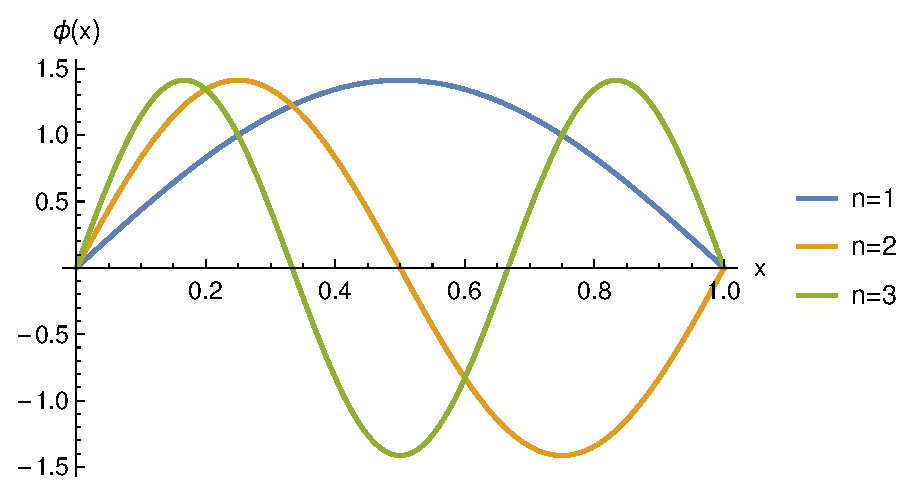
\includegraphics[width=0.65\textwidth]{box_wave.eps}
  \caption{Particle in a box wavefunction for
    the three energy levels ($i=1,2,3$).}
  \label{fig:box_wave}
\end{figure}

{\color{blue} The sums of the energies for 1, 2, and 3 levels are given
  \begin{align}
    E_1 + E_2 & = \frac{5\pi^2}{2} \\
    E_1 + E_2 + E_3 & = 7\pi^2
  \end{align}
  The densities ($n_j(x)$) for 1, 2, and 3 same-spin fermions ($j=1,2,3$)
  in the box are the sum of the $\phi_i(x)^2$
  \begin{align}
    n_1(x) & = \phi_1(x)^2 \\
    n_2(x) & = \phi_1(x)^2 + \phi_2(x)^2 \\
    n_3(x) & = \phi_1(x)^2 + \phi_2(x)^2 + \phi_3(x)^2
  \end{align}
}
\begin{figure}[H]
  \centering
  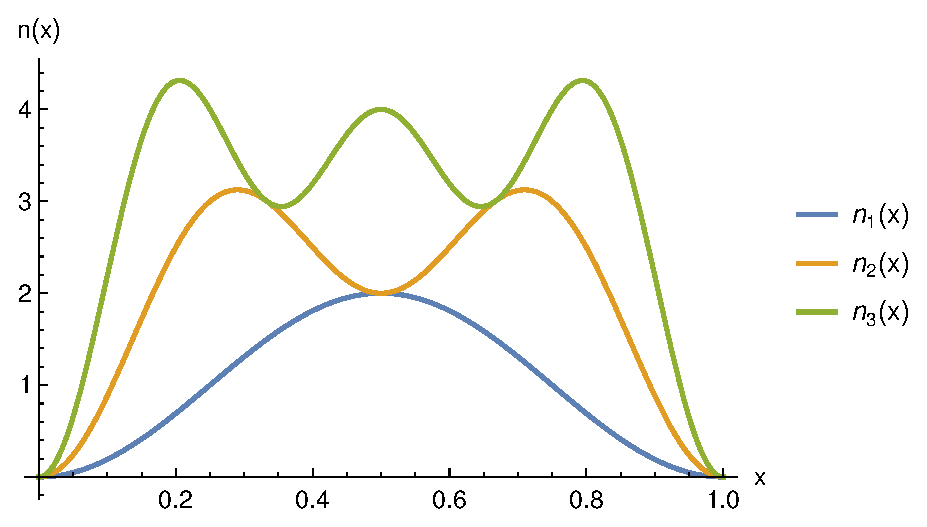
\includegraphics[width=0.65\textwidth]{box_dens.eps}
  \caption{Densities for 1, 2, and 3 fermions same-spin are plotted.}
  \label{fig:box_dens}
\end{figure}

\noindent b) Solve the Euler-Lagrange equation with the TF approximation
to the kinetic energy to find the relation between $N$ and $\mu$.  Solve
for the mininimizing density, and plot it on your density plots.  Comment
on the errors made by this approximate density, and how the error behaves
as $N$ grows.  Calculate the integral of $n^2(x)$ for $N=1,2,3$, both exactly
and approximately and comment as $N$ grows.
\\

{\color{blue}
  \begin{align}
    L[n,\mu] & = T^{\text{TF}}[n] -\mu \int dx\, n(x) \\
    \frac{\delta L}{\delta n} & = \frac{\delta T^{\text{TF}}[n]}{\delta n} - \mu = 0 \\
    \frac{\delta T^{\text{TF}}[n]}{\delta n} & = \frac{\pi^2n(x)^2}{2} = \mu \\
    \mu & = \frac{\pi^2N^2}{2}
  \end{align}

  Since the multiplier $\mu$ has been determined in terms of $N$, the
  approximate minimizing density is given
  \begin{align}
    n(x) = N.
  \end{align}

  The integral of $n^2(x)$ for $N=1,2,3$ for the approximate TF density
  becomes worse with increasing $N$ and the $n^2(x)$ integral is $N^2$
  while the exact density yields the correct number of electrons at
  $N=1,2,3$.}

  \begin{figure}[H]
    \centering
    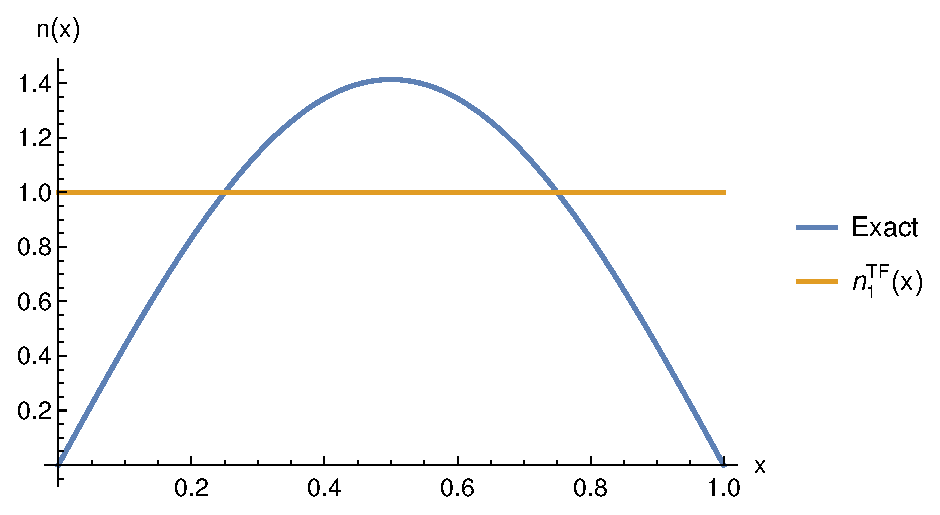
\includegraphics[width=0.47\textwidth]{tf_onepart.eps}
    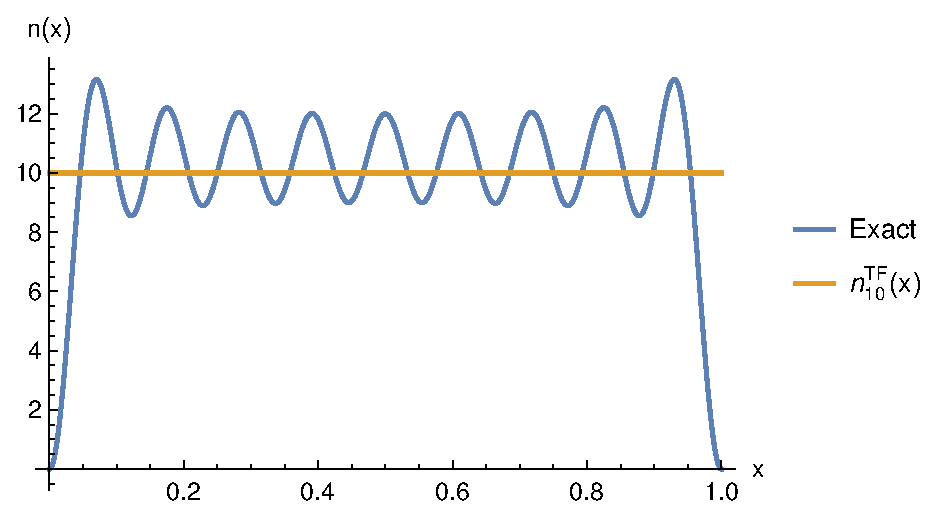
\includegraphics[width=0.47\textwidth]{tf_tenpart.eps}
    \caption{Thomas-Fermi minimizing density and exact density given
      for 1 and 10 particles.}
    \label{fig:tf_dens}
  \end{figure}

{\color{blue} With increasing $N$, the TF density looks closer to describing
  exact density.}
\\

\noindent c) Make a table of the exact and approximate kinetic energies
for each $N$ and report the percentage error.  Comment on the absolute error
and percent error as $N$ grows.

\begin{table}[H]
  \caption{Comparison between exact and approximate
    Thomas--Fermi kinetic energies with respect to increasing $N$ particles.}
  \centering
  \begin{tabular}{crrr}
    $N$ & $T^{\text{exact}}$ & $T^{\text{TF}}[n_{\text{approx}}]$ & Error ($\%$) \\
    \hline
     1 &4.935& 1.645 & -66.667 \\
     2 &24.674& 13.160 & -46.667 \\
     3 &69.0872& 44.413 &-35.714 \\
     4 &148.044& 105.276 &-28.889 \\
     5 &271.414& 205.617 &-24.242 \\
     6 &449.067& 355.306 &-20.879 \\
     7 &690.872& 564.212 &-18.333 \\
     8 &1006.7& 842.206 & -16.340 \\
     9 &1406.42& 1199.16 &-14.737 \\
     10&1899.9& 1644.93 & -13.420 \\
     11&2497.01& 2189.41 &-12.319 \\
     12&3207.62& 2842.45 &-11.385 \\
     13&4041.6& 3613.92 & -10.582 \\
     14&5008.82& 4513.7 & -9.885  \\
     15&6119.15& 5551.65 &-9.274  \\
    100&1.6697 $\times$ 10$^6$ & 1.6449$\times$ 10$^6$& -1.4826
  \end{tabular}
\end{table}

{\color{blue} Approximate TF kinetic energy improves with increasing $N$. The
  TF consistently underestimate the kinetic energies.
}
\\

\noindent d) Now calculate the TF kinetic energy on the exact densities and
add the results to the table, including errors and comment as $N$ grows.
What do you conclude is the main  source of error in the self-consistent
TF calculation?

\begin{table}[H]
  \caption{Comparison between exact kinetic energy and Thomas--Fermi
    kinetic energy on exact density.}
  \centering
  \begin{tabular}{crrr}
    $N$ & $T^{\text{exact}}$ & $T^{\text{TF}}[n_{\text{exact}}]$ & Error ($\%$) \\
    \hline
   1& 4.9348& 4.11234& -16.667 \\
   2& 24.674& 21.7954& -11.667 \\
   3& 69.0872& 62.9187& -8.929 \\
   4& 148.044& 137.352& -7.222 \\
   5& 271.414& 254.965& -6.061 \\
   6& 449.067& 425.627& -5.220 \\
   7& 690.872& 659.207& -4.583 \\
   8& 1006.7& 965.576& -4.085 \\
   9& 1406.42& 1354.6& -3.684 \\
   10& 1899.9& 1836.16& -3.355 \\
   11& 2497.01& 2420.11& -3.080 \\
   12& 3207.62& 3116.33& -2.846 \\
   13& 4041.6& 3934.68& -2.646 \\
   14& 5008.82& 4885.04& -2.471 \\
   15& 6119.15& 5977.28& -2.319 \\
  100& 1.6697$\times$ 10$^6$ & 1.6635$\times$ 10$^6$& -0.370
  \end{tabular}
\end{table}

{\color{blue} Errors are even smaller with the exact density. One main source
  of the error arise from a poor density.
}
\\

\noindent e) Remake your table to report eigenvalues, by calculating the
difference between having $N$ and $N-1$ particles in the box, and calculate
errors for both self-consistent TF and TF on exact densities.

\begin{table}[H]
  \caption{Kinetic energy difference computed between $N$ and $N-1$ state
    ($\epsilon_{N-1,N}$).}
  \centering
  \begin{tabular}{crrrrr}
    $\epsilon_{N-1,N}$ & $T^{\text{exact}}$ & $T^{\text{scf,TF}}$ &
    Error ($\%$) & $T^{\text{TF}}[n_{\text{exact}}]$ & Error ($\%$) \\
    \hline
     $\epsilon_{1,2}$&  19.739 & 11.5145 & -41.667 & 17.683 & -10.417 \\
     $\epsilon_{2,3}$&  44.413 & 31.2537 & -29.630 & 41.123 & -7.407 \\
     $\epsilon_{3,4}$&  78.957 & 60.8626 & -22.917 & 74.433 & -5.730 \\
     $\epsilon_{4,5}$&  123.370 & 100.341 & -18.667 & 117.613 & -4.667 \\
     $\epsilon_{5,6}$&  177.653 & 149.689 & -15.741 & 170.662 & -3.935 \\
     $\epsilon_{6,7}$&  241.805 & 208.907 & -13.605 & 233.581 & -3.401 \\
     $\epsilon_{7,8}$&  315.827 & 277.994 & -11.979 & 306.369 & -2.995 \\
     $\epsilon_{8,9}$&  399.719 & 356.951 & -10.700 & 389.027 & -2.675 \\
     $\epsilon_{9,10}$&  493.480 & 445.777 & -9.667 & 481.554 & -2.417 \\
     $\epsilon_{10,11}$&  597.111 & 544.473 & -8.815 & 583.952 & -2.204 \\
     $\epsilon_{11,12}$&  710.612 & 653.039 & -8.102 & 696.218 & -2.025 \\
     $\epsilon_{12,13}$&  833.982 & 771.474 & -7.495 & 818.355 & -1.874 \\
     $\epsilon_{13,14}$&  967.221 & 899.779 & -6.973 & 950.361 & -1.743 \\
     $\epsilon_{14,15}$&  1110.330 & 1037.95 & -6.519 & 1092.240 & -1.630 \\
     $\epsilon_{99,100}$& 49348. & 48856.2 & -0.997 & 49225.1 & -0.249
  \end{tabular}
\end{table}

\noindent f) Deduce formulas for $E_N$ for the exact and two approximate sets
of numbers, and then add $N=100$ to your table.   What aspect of the formulas
show that TF becomes relatively exact as $N$ gets large?  (Hint:  In every case,
the formulas are cubic polynomials in $N$ with no constant term (why?) whose
coefficients could be found by fitting to 3 values of $N$.)

{\color{blue}
  \begin{align}
    E_N^{\text{exact}} & = \frac{\pi^2N^3}{6} + \frac{\pi^2N^2}{4} + \frac{\pi^2N}{12} \\
    E_N^{\text{TF}} & = \frac{\pi^2N^3}{6} + \frac{\pi^2N^2}{4} + \frac{\pi^2N}{12} \\
    E_N^{\text{scf,TF}} & = \frac{\pi^2N^3}{6}
  \end{align}
}

\pagebreak

\section*{Harmonic oscillators in DFT}

\noindent a) For the harmonic oscillator $v(x)=x^2/2$, write the formula for
the TF density in terms of $\mu$.
{\color{blue}
  \begin{align}
    L[n,\mu] & = T^{\text{TF}}[n] + \int dx\, v(x)n(x) -\mu\int dx\, n(x)\\
    \frac{\delta L}{\delta n} & = \frac{\delta T^{\text{TF}}[n]}{\delta n}
      v(x) - \mu = 0 \\
    n^{\text{TF}}(x) & = \frac{\sqrt{2(\mu-\frac{1}{2}x^2)}}{\pi}
  \end{align}
}

\noindent b) By doing the integral between the turning points, find a formula
for $N$ as a function of $\mu$.
\\

{\color{blue} $\mu = N$}
\\

\noindent c) Get formulas for $T_N$ and $E_N$.    
{\color{blue}
  \begin{align*}
  T_N & = 2\frac{\pi^2}{6}\int_0^{\sqrt{2N}}dx\,
  \Bigg(\frac{\sqrt{2(N-\frac{1}{2}x^2)}}{\pi}\Bigg)^3 \\
  & = \frac{N^2}{4} \\
  V_N & = \frac{N^2}{4} \\
  E_N & = \frac{N^2}{2}
  \end{align*}
}

\noindent d) By subtracting $N-1$ from $N$, deduce a formula for the $N$-th
energy level.  What is its error?
\\

{\color{blue} $E^{\text{TF}}_N - E^{\text{TF}}_{N-1} = N-1/2$ which is exact}
\\

\noindent e) For $N=1,2,3$, plot both the exact and the approximate densities
of the harmonic well. Why would the phrase "getting the right answer for the
wrong reason" come to mind?
\\
\begin{figure}[H]
  \centering
  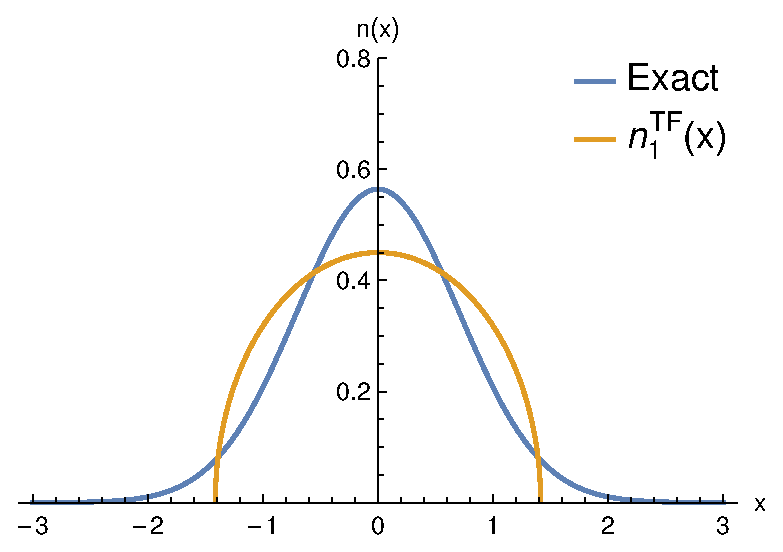
\includegraphics[width=0.325\textwidth]{ho1_compare.eps}
  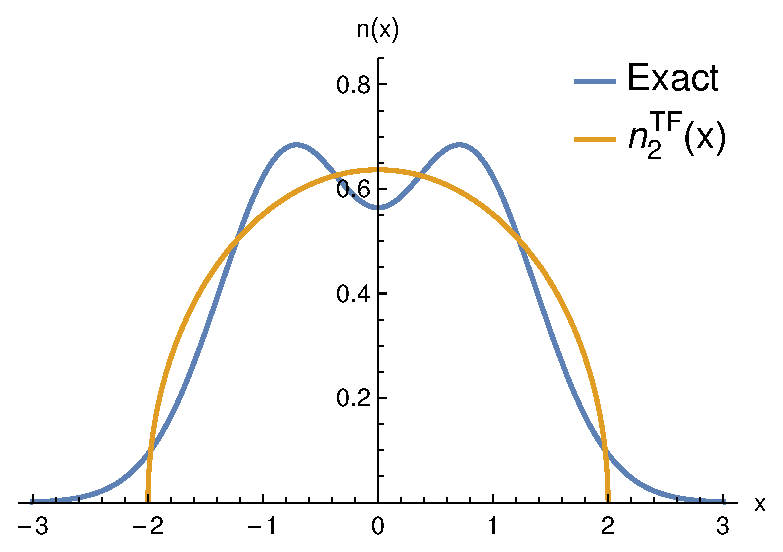
\includegraphics[width=0.325\textwidth]{ho2_compare.eps}
  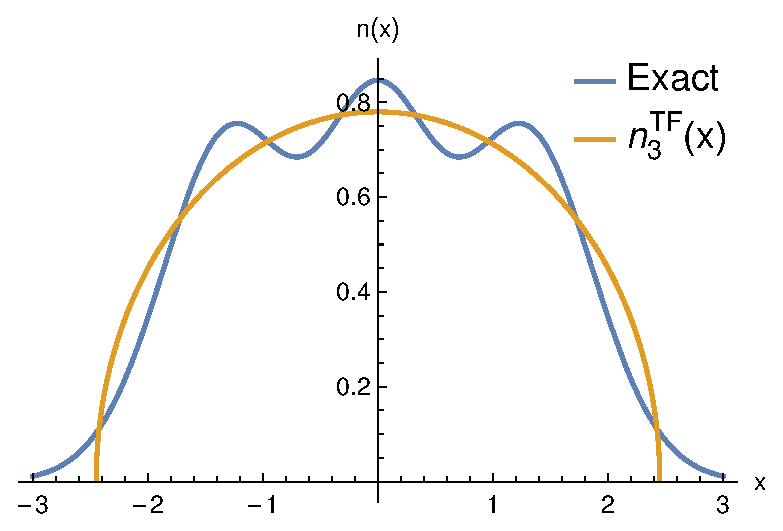
\includegraphics[width=0.325\textwidth]{ho3_compare.eps}
  \caption{Exact and the approximate densities of the harmonic well for
    1, 2, and 3 particles (from left to right).}
\end{figure}

\noindent f) Calculate the integral of $n^2(x)$ for $N=1,2,3$ both exactly
and approximately and comment on trends of errors with $N$.
\\
 
{\color{blue} Both the exact and TF densities yield the same integral of
  $n^2(x)$ for $N=1,2,3$ which correspond to the number of electrons.
}
\pagebreak
\section*{Morse oscillators in DFT}

\noindent a) For the Morse potential given for the diatomics problem, 
$$E^{TF}_N = - N V_0 (1-y+y^2/3)$$
where $y=N/\alpha$.  Deduce a formula for individual eigenvalues.
{\color{blue}
  \begin{align}
    E^{TF}_N - E^{TF}_{N-1} & = - \frac{V_0(N^2-3N\alpha+3\alpha^2)}{3\alpha^2}
  \end{align}
}

\noindent b) For your parameters for H$_2$ modelled as a Morse potential. 
List the exact and approximate vibrational energy levels.  Comment on where the
largest errors are.
\\

\begin{table}[

\noindent c) What happens for D$_2$?  Does the TF result do better or worse than in H$_2$?  Does
it depend on which eigenvalues you look at?  Why does it get better or worse?
\\

\end{document}
